\chapter{Comparison to Run-I Results}
\textbf{Note:} This section has been written assuming an integrated luminosity of 2.1\fbinv at 13\,\TeV. It has not been updated to \fullLumi (since pre-approval).

We show that the sensitivity of our current analysis is plausible, given the improvements that were made in comparison to the Run I analysis. To this end, we compute expected limits starting from a mock-up analysis setup that is very similar to the Run I analysis. As we then add various improvements, we arrive at the limit shown in Section~\ref{sec:Interpretation}. The investigations are done using the signal mass point with $m_\Sigma = 340\,\GeV$ and described in the following; a summary is presented in Table~\ref{tab:improvements}.

We extract the expected $r$-value from Figure 2 in the Run I PAS, \cite{CMS-PAS-EXO-14-001}. We find $\frac{\sigma_\textrm{experimental} \cdot \textrm{BR}}{\sigma_\textrm{theory} \cdot \textrm{BR}} = \frac{14\,\textrm{fb}}{4.3\,\textrm{fb}} = 3.26$. Note that the theory cross-section here contains a k-factor of 1.35, which we do not currently use in our analysis as we await the official samples. The figure of merit is thus $r_\textrm{exp}^{8\TeV} = 3.26 \cdot 1.35 = 4.40$.

To relate this 8\,\TeV number to the current 13\,\TeV dataset with 2.1\fbinv, we divide the $r$-value by the cross-section ratio $\frac{\sigma(13\,\TeV)}{\sigma(8\,\TeV)} = 2.99$ and multiply by a correction factor for the different luminosities, $\sqrt{19.5/2.1}$. We thus find that the Run I analysis sensitivity corresponds to an expected r-value of $r_\textrm{exp} = 4.49$ at 13\,\TeV.

Using a mock-up Run I analysis setup based on charge binning with the current 13\,\TeV dataset (2.1\fbinv), we actually find an expected r-value of $r_\textrm{exp} = 6.20$ (exactly 3 electrons or muons, \pt thresholds at 30/20/20\,\GeV, $\MET > 50\,\GeV$, $\HT < 150\,\GeV$, \Z veto, AIC veto). The two charge bins that this limit is based on are displayed in Fig.~\ref{fig:app:RunI}.

6.20 is worse than 4.49 by 38\,\%. We ascribe this difference -- which is in the conservative direction in any case -- to the various approximations we have made to mimic the Run I analysis. Also, the Run I analysis used somewhat finer flavor-dependent binning scheme.

\begin{figure}[h]
\begin{center}
	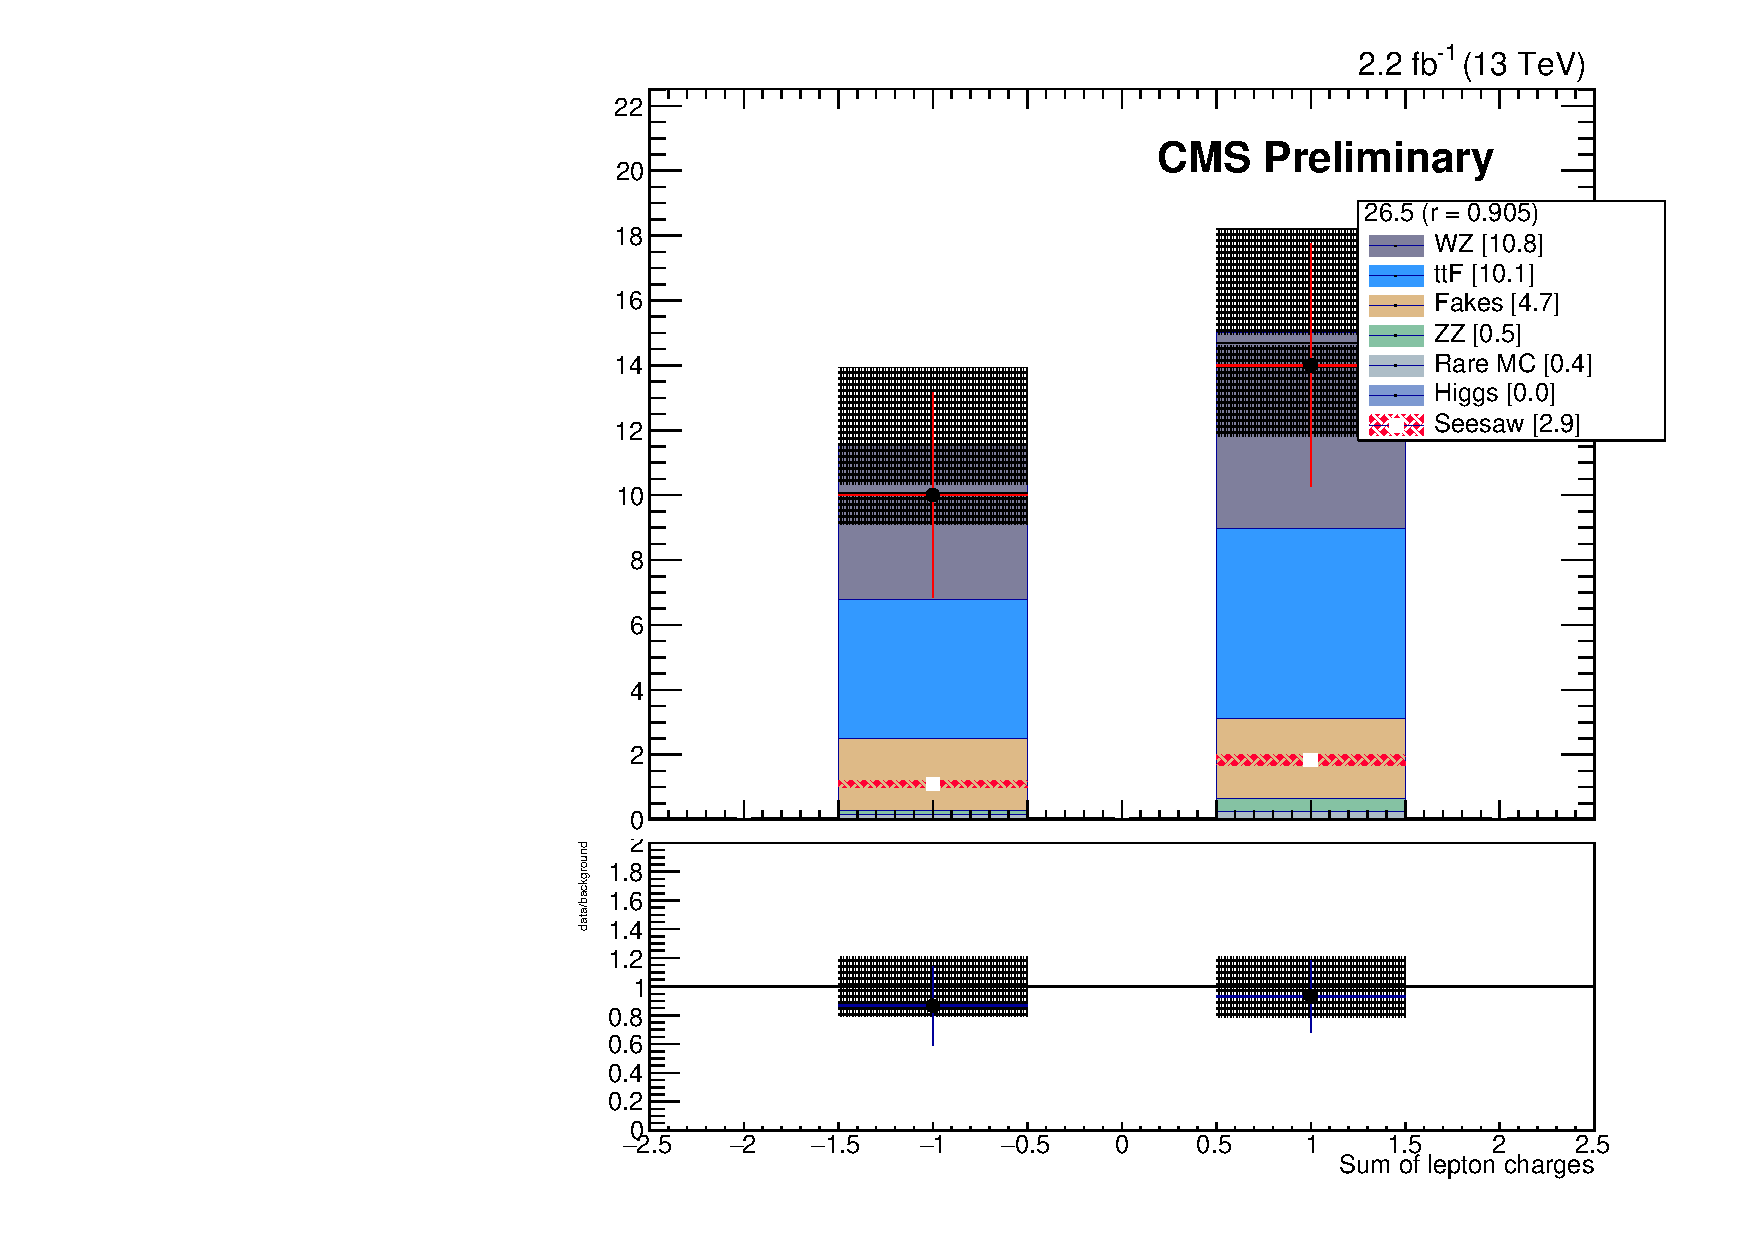
\includegraphics[width=.7\textwidth]{Appendix/L3Tau0_Q}\
	\caption{Bins of lepton charge sum used in mock-up Run I result, with 13\,\TeV dataset and background estimates (3 leptons only)
	\label{fig:app:RunI}}
\end{center}
\end{figure}

Now, starting from $r_\textrm{exp} = 6.20$, we show how various improvements lead to the $r$-value of 0.87 which is presented in Section~\ref{sec:Interpretation}. Table~\ref{tab:improvements} shows the details of how the limits improve.

\begin{table}[h]
\centering
\caption{Sensitivity improvements compared to the Run I analysis} \label{tab:improvements}
\begin{tabular}{c c l}
\hline\hline
$r_\textrm{exp}$ & Improvement & Step \\
\hline
\hline
3.26 & & Run I result \\
4.40 & & Run I result without k-factor \\
4.49 & & Run I result translated to 2.1\fbinv at 13\,\TeV\\
\hline
6.20 & -- & Run I result with Run I mock-up analysis setup \\
5.30 & 15\,\% & mock-up analysis with current \pt thresholds and kinematic cuts \\
3.55 & 33\,\% & adding signal with Higgs decay modes \\
1.14 & 68\,\% & switching to $L_\textrm{T} + \MET$ binning (= current search with only 3 leptons) \\
0.87 & 24\,\% & adding 4-lepton channels (= current result) \\
\end{tabular}
\end{table}
